\chapter{Dataset}
\label{sq:dataset}

In this section, we introduce a new dataset for the interactive fashion outfit recommendation task. We also report our findings on the importance of the question selection through the analysis of the developed dataset.

\section{Source Data}
Polyvore\footnote{\url{https://www.polyvore.com/}} was a fashion commerce website, 
which allowed users to upload outfits they liked
and provided several functions to facilitate users' exploration of fashion items and outfits. 
Since 2015, the data from Polyvore has been widely used in various fashion researches~\cite{hu2015collaborative, li2017mining, vaccaro2016elements, chen2019pog}.
Our dataset was constructed with the dataset developed by Han et al.~\cite{han2017learning}, 
which consists of 21,889 outfits with 164,379 items.
Each outfit contains multiple items and rich metadata such as  the number of likes, hashtags, etc. 
Moreover, each item also has rich multimodal information, such as the description, image, and category. 
Note that outfits were developed by designers and used as 
ground truth in the outfit recommendation tasks
such as ``fill in the blank'' and compatibility prediction. 

\section{Assumption for Simulation}
To the best of our knowledge, there is no previous study on interactive fashion outfit recommender systems, and the Polyvore dataset lacks user-system interaction information. 
To generate a dataset for interactive fashion recommender systems, 
we propose an assumption that
there is a user who desires each outfit in the Polyvore dataset,
and the interactive recommender system
cannot identify the exact outfit the user is looking for,
but can identify candidate items for each category,
one of which is a part of the desired outfit.
Table \ref{tb:example_questions} shows an example of 
the assumed situations.
For three categories ``Tops'',
``Bottoms'', and ``Shoes'',
five fashion items are retrieved for a given user, respectively.
Each of the fashion items is potentially relevant,
but only a fashion item in each category is a part of the desired outfit (e.g., T1, B1, and S1 forms the desired outfit). 
A set of items from each category can be used as a question,
as they are potentially relevant items,
and the recommender system needs to identify a question to be asked at each round.
In the example of Table \ref{tb:example_questions},
the recommender system can ask one of three questions 
$Q_1=\{{\rm T1}, \ldots, {\rm T5}\}$, $Q_2=\{{\rm B1}, \ldots, {\rm B5}\}$, and $Q_3=\{{\rm S1}, \ldots, {\rm S5}\}$.
When $Q_1$ is presented to the user, 
we assume that T1 is chosen by the user as an answer to $Q_1$.
Therefore, we can simulate users' responses to some questions 
and automatically evaluate the performance of question selection algorithms.
Note that the recommender system cannot 
identify the desired outfit and 
which item is answered by the user before the question is asked.


\begin{table}[t]
  \centering
  \caption{Example of questions in our dataset.}
  \begin{tabular}{lccc}
  \toprule 
    Question&$Q_1$&$Q_2$&$Q_3$\\
    \midrule
    Category&Tops&Bottoms&Shoes\\
    \midrule
    Outfit&T1&B1&S1\\
    \midrule
    &T2&B2&S2\\
    &T3&B3&S3\\
    &T4&B4&S4\\
    &T5&B5&S5\\
  \bottomrule
  \end{tabular}
  \label{tb:example_questions}
\end{table}

The task definition of the interactive fashion outfit recommendation becomes a little more specific when our dataset is used.
Given a user $U$ who prefers to an outfit $O$ as well as a question $Q$,
$U$ returns $a \in Q$ as an answer such that $a \in O$.
Moreover, a set of questions $\mathcal{Q}_U$ is prepared for each user $U$, from which the question selection algorithm is expected to choose the most appropriate question at each time step.
Thus, $\mathcal{Q}$ in Equation \ref{eq:question_value} is replaced with $\mathcal{Q}_U$, 
meaning that there are, say, six candidate questions for each user.

Although this assumption enables us to simulate user-system interactions for fashion outfit recommendation, there are two limitations of this approach. 
One is the assumption that we can prepare a set of items,
one of which is relevant to the user.
Its feasibility highly depends on the fashion recommendation algorithm
and can be approximated by the HIT@$k$ metric (1 if the top-$k$ items contain a relevant item; otherwise 0).
This limitation can be alleviated if the fashion recommendation algorithm is improved.
The other limitation is that questions are pre-defined and not purely generated by the interactive recommendation system.
This might prevent us from accurately evaluating the ability 
of interactive fashion outfit recommender systems,
since they may be able to generate better questions and achieve higher recommendation accuracy with better interactions.
Whereas, such systems must be able to correctly 
identify the best question among candidates and achieve relatively higher performances than the others.
This type of assumption has been often posed in 
dialogue generation tasks (e.g., \cite{shang2016overview}). 

\section{Question Generation}

As discussed in the previous subsection, the quality of questions is vital for realistic question-answering simulation. 
A qualified question should consist of relevant items,
any of which can be a part of reasonable outfits. 
The key idea to guarantee the question quality is 
to choose potentially relevant items as a part of desired outfits. 
Since we can access the complete outfit in developing questions,
we can find alternatives to a particular item in the outfit
by solving the ``fill in the blank'' task given the other items in the outfit. 

Specifically, first, we choose an outfit from the Polyvore dataset,
e.g., $O = \left\{{\rm T1}, {\rm B1}, {\rm S1} \right\}$ in Table \ref{tb:example_questions}.
To generate a question of ``Tops,''
we input B1 and S1 to a fashion compatibility model
and find suitable items that {\it fill in the blank}, e.g., T2, T3, T4, and T5.
A question $Q_1$ can be composed of the original fashion item T1
as well as the output fashion items T2 -- T5.
Then, we iterate this process for all the fashion items in the outfit to generate a question for each category.
We assume that the fashion compatibility model
can identify comparably suitable fashion items for the other items,
which are all reasonable options for the user. 


Firstly, we initialize a question with one of the fashion items $o \in O$.
Secondly, the algorithm finds $k-1$ fashion items to complete the question.
A fashion compatibility model $f$, which takes an incomplete outfit and another fashion item to return the compatibility score of the fashion item, is used to find the $k-1$ most compatible fashion items for $O \setminus \{ o \}$. 
Iterating this procedure, we finally obtain $\mathcal{Q}_U$ containing $|O|$ questions, each of which corresponds to each fashion item in $O$.


As a fashion compatibility model $f$, we used the Bidirectional LSTMs model to calculate the compatibility of fashion outfits, which was developed by Han et al.~\cite{han2017learning}. 
The number of items in a question, $k$, is set to 5 for ease of users' choices. 


\section{Analysis}
\label{sq:analysis}

\begin{table}[t]
\caption{Dataset statistics.}
\centering
\begin{tabular}{ccc}
\toprule
\# Question sets&\# Questions&\# Unique items\\
\midrule
2,758&16,768&16,768\\
\bottomrule
\end{tabular}
\label{dataset-basic-stats}
\end{table}

Table \ref{dataset-basic-stats} shows the basic statistics of the dataset.
In the developed dataset, the items are grouped in over 380 different categories.
As the number of items in some categories is lower than five, 
we excluded the categories with small volumes to ensure that each question can contain five items.
Finally, we obtained 2,758 question sets, 16,768 questions, and 16,768 unique items.
As outfits from the Polyvore dataset may have different numbers of items,
the question sets generated based on outfits also have different amounts of questions.
Table \ref{dataset-sets-stats} reports the statistics of the size of question sets. 
Over 59.8\% of the question sets contain at least six questions. 
The average number of questions per question set is 6.08.

\begin{table}[t]
\caption{Number of question sets with the different number of questions.}
\centering
\begin{tabular}{cc}
\toprule
Size of question sets & \# Question sets \\ \midrule
4                & 526                 \\
5                & 580                 \\ 
6                & 548                 \\ 
7                & 356                 \\ 
8                & 748                 \\ \bottomrule
\end{tabular}
\label{dataset-sets-stats}
\end{table}

We then investigated what questions are likely to be effective in the interactive fashion outfit recommendation task.
To this end, we tested various questions and computed the effectiveness measure of the recommended outfit. 
More specifically, we assumed a situation where only a question had already been asked and answered by a user. 
All the possible questions were asked in the simulation as the second question.
The effectiveness of the second question was evaluated by the fashion outfit recommendation,
in which candidate outfits are limited to those consisting of the answers to the first and second questions as well as an item from another question. 
For example, given a set of questions $\mathcal{Q} = \left\{ Q_1, Q_2, Q_3 \right\}$, let $Q_1$ be the question already asked.
We then ask $Q_2$ and simulate the user's answer to this question.
Based on the question-answering history $H_2 = \{(Q_1, a_1), (Q_2, a_2)\}$, 
the outfit recommendation algorithm $R$
ranks only the fashion outfits consisting of $a_1$ and $a_2$ as well as an item in $Q_3 = \{i_1, i_2\}$, i.e., $\{a_1, a_2, i_1 \}$ and $\{a_1, a_2, i_2 \}$.
The effectiveness of $Q_2$ is the reciprocal rank of a relevant outfit in the outfit ranking,
where the relevant outfit is defined as the one constituting $O$ (an item set from which $\mathcal{Q}$ was generated).
To develop the recommendation algorithm $R$, we used the same fashion compatibility model $f$ used to produce questions in the dataset.
The fashion compatibility model solves the ``fill in the blank'' problem for given items (e.g., $a_1$ and $a_2$), and ranks items to form a ranked list of outfits.
For example, given a ranked list of items produced by the fashion compatibility model,
$(i_2, i_1)$, the outfit ranking is obtained as follows: 
$(\{a_1, a_2, i_2\}, \{a_1, a_2, i_1\})$.


\begin{figure}
  \centering
  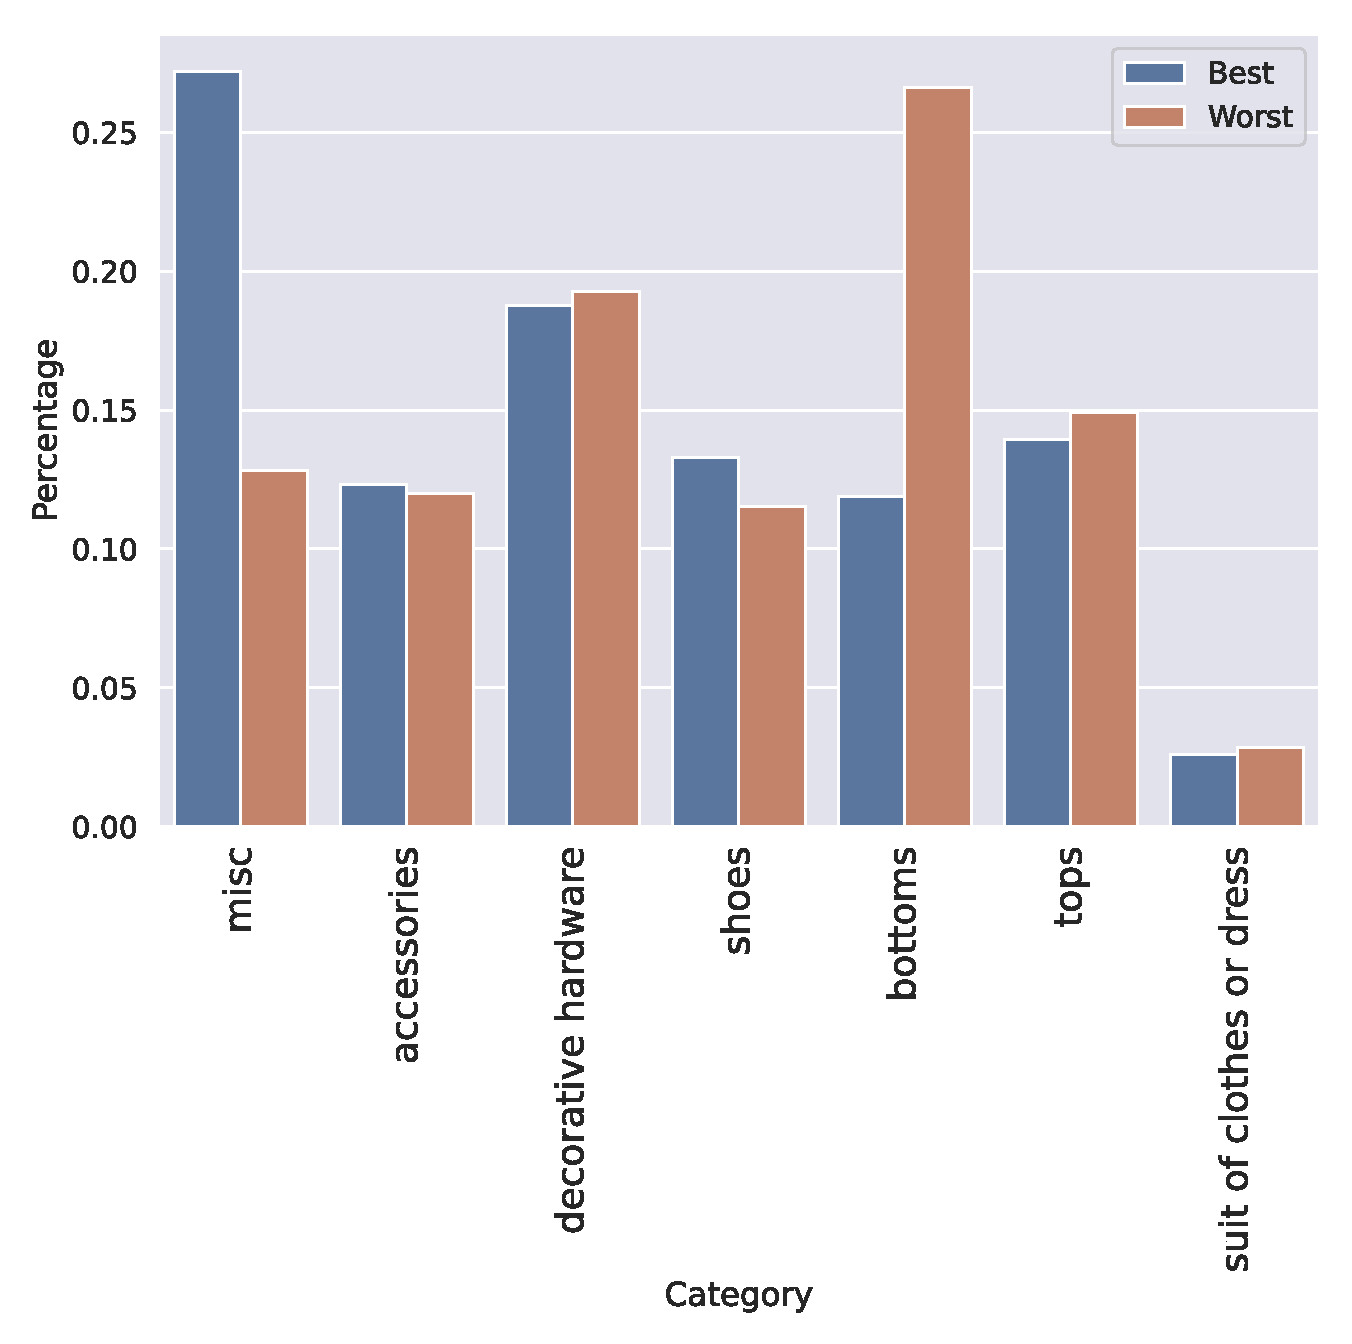
\includegraphics[width=\linewidth]{figures/category_stats_long.eps}
  \caption{Percentage of the best and worst questions in each category.}
  \label{category-stats}
\end{figure}

\begin{figure}
  \centering
  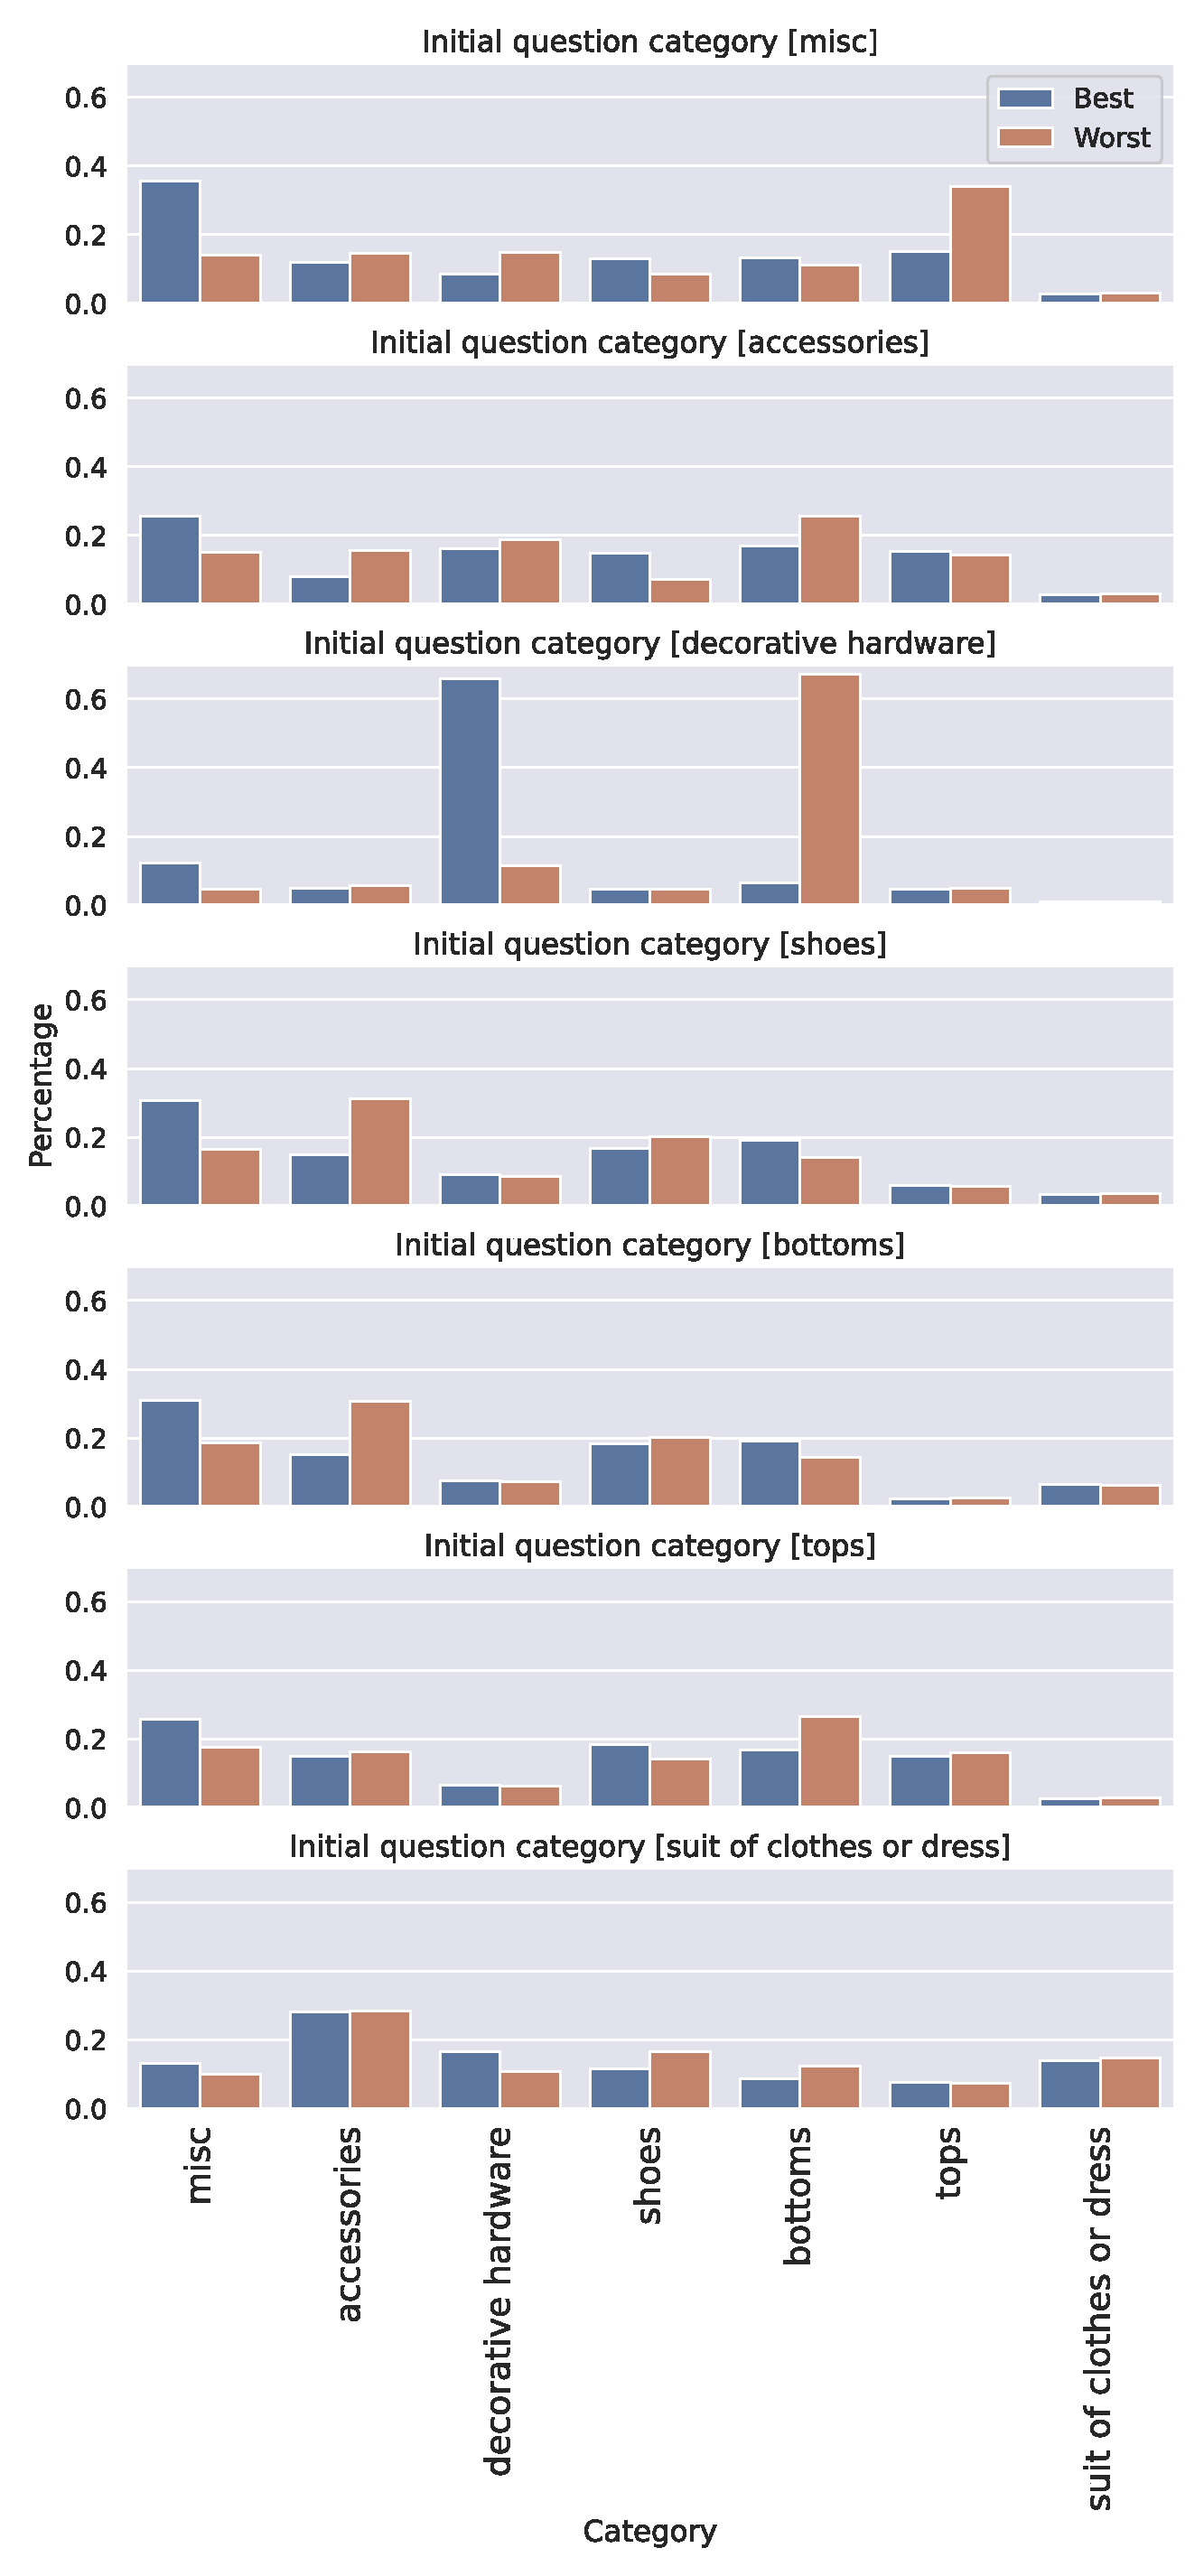
\includegraphics[width=0.6\linewidth]{figures/category_stats_init_long.eps}
  \caption{Percentage of the best and worst questions in each category with different categories of the initial question.}
  \label{category-stats-init}
\end{figure}

\begin{table}[t]
\caption{Effectiveness of the best and worst questions. ``All'' indicates that of all the questions.}
\centering
\begin{tabular}{ccc}
\toprule
 All   & Best & Worst \\ \midrule
 0.397 & 0.602        & 0.243         \\
\bottomrule
\end{tabular}
\label{tb:best_worst}
\end{table}

We first show the average effectiveness of the best and worst questions in Table \ref{tb:best_worst}.
A question is the best question if the recommendation with the question achieved the highest effectiveness among the other questions in a question set. 
The worst question is defined similarly. 
We found that there is a large performance gap between the best and worst questions.
This result suggests that the question selection algorithm has a large impact on the outfit recommendation performance. 

We then show what category of questions led to effective outfit  recommendations.
Figure \ref{category-stats} shows the percentage of the best and worst questions in each category.
Since there are over 380 different item categories in the developed dataset, 
we manually organized those categories into seven groups for our analysis: \textit{a suit of clothes or dress}, \textit{tops}, \textit{bottoms}, \textit{shoes}, \textit{accessories}, \textit{decorative hardware}, and \textit{miscellaneous}. 
The figure shows large differences across the categories:
the category such as \textit{miscellaneous} shows a high probability of being the best question, while questions from the \textit{bottoms} category are unlikely to receive helpful users' feedback.


Figure \ref{category-stats-init} reports the percentage of 
the best and worst questions in each category,
with different categories of {\it initial questions}. 
Recall that we assumed a question had already been asked in this simulation: 
this question is defined as the initial question.
With the initial question in different categories, 
the effectiveness of questions changes significantly.
For example, following a question about decorative hardware with another question may improve the accuracy of future predictions.
There are two possible reasons for these uneven performances across categories: 
(1) some categories (e.g., bottoms) are not informative probably because of a limited number of variations in the category.
(2) the consistency of some categories can be strongly required to form good outfits. 
For example, the style of bottoms and shoes must be the same. 
In this case, it is not very informative to ask questions regarding shoes when the question about bottoms is already asked. 

\begin{table}[t]
\caption{Average similarity to the previous question and heterogeneity of the best and worst questions.
``All'' indicates those of all the questions.}
\centering
\begin{tabular}{lccc}
\toprule
                       & All   & Best & Worst \\ \midrule
Similarity & 0.352 & 0.365        & 0.307         \\
Heterogeneity            & 2.484 & 2.460        & 2.546         \\
\bottomrule
\end{tabular}
\label{dis-sim}
\end{table}

We further investigated the similarity between the previous question and best/worst question,
and the heterogeneity of the best and worst questions.
The similarity between two questions is defined as the cosine similarity between the question embeddings:
\begin{eqnarray}
{\rm sim}(Q_a, Q_b) = \frac{\mathbf{Q}_{a} \cdot \mathbf{Q}_{b}}{\|\mathbf{Q}_{a}\|\|\mathbf{Q}_{b}\|}
\label{eq:sim}
\end{eqnarray}
Here, a question embedding $\mathbf{Q}_{a}$ is defined as the mean of the embeddings of items in the question $Q_a$:
$\mathbf{Q}_a = \frac{1}{|Q_a|} \sum_{i \in Q_a} \mathbf{i}$,
where $\mathbf{i}$ is an embedding of the item $i$,
which was generated with a visual-semantic embedding model consisting of visual features extracted from ResNet~\cite{he2016deep} and semantic feature from Word2Vec~\cite{mikolov2013efficient} model.

The heterogeneity of a question indicates to what extent different items constitute the question,
and is defined as the mean of euclidean distances between all item pairs:
\begin{eqnarray}
{\rm het}(Q) = \frac{1}{k(k-1)} \sum_{i_a, i_b \in Q} \| \mathbf{i}_a - \mathbf{i}_b \| 
\end{eqnarray}

Table \ref{dis-sim} demonstrates that the best question has higher similarity to the previous question and lower heterogeneity than the average and worst questions.
These findings can be explained from the viewpoint of informativeness of questions.
In active learning~\cite{settles2009active}, 
it is more informative to receive labels for similar examples that are difficult to distinguish. 
This principle could be applied to our case: letting the user choose from similar questions
(i.e., questions similar to the previous question or those consisting of similar items) is more effective to distinguish preferred items and the others.


In summary, we discovered that (1) the question selection has a significant impact on recommendation performance, (2) the category of fashion items in the question has an impact on recommendation performance,
and (3) effective questions are likely to be homogeneous and similar to the previous question. 
